\documentclass[UTF8]{ctexart}
\usepackage{graphicx}
\usepackage{amssymb}
\usepackage{subfiles}
\usepackage{amsmath}
\usepackage[margin=1in]{geometry}
\begin{document}
\section{Numerical result and discussion-数值结果和讨论}
\paragraph{\quad}In this section, firstly, the accuracy and convergence 
            of the adopted multiphase Riemann-SPH method are validated 
            through the test of the slamming of a flat plate. Then, 
            the influences of the air cushion and the plate length on the 
            slamming load are discussed. Finally, focusing on the air-cushion 
            effect in the water entry, a complex engineering problem, i. e., 
            the slamming of the LNG tank insulation panel is simulated, and the 
            influences of the impact velocity and deadrise angle on slamming load 
            characteristics are analyzed.
\paragraph{\quad}本节通过平板砰击实验验证了采用的黎曼-SPH方法的精确性和收敛性。随后,讨论了
                气垫效应和板长对砰击载荷的影响。最后,重点研究了入水过程中的气垫效应,
                模拟了一个复杂的工程问题,即LNG船绝缘板的砰击,并分析了砰击速度和静升角
                对砰击载荷特性的影响。

\subsection{slamming of flat plate-平板砰击}
\subsubsection{Validation-验证}
\paragraph{\quad}This subsection aims to verify the accuracy and convergence 
                of the adopted SPH method by the test of water slamming of 
                flat plate which is carried out by Ma et al. (2016). The sketch 
                of the numerical model is shown in Fig. 1, in which$ M$,$ l $and $U_{impact}$ 
                stand for the mass, the length and the impact velocity of the plate, 
                respectively.$ H $and$ W $denote the depth and width of water domain, 
                respectively. In the experiment, the plate has the length of$ l = 0.25 m$ 
                and the mass of $M = 32 kg$. This plate is released at rest initially and 
                falls freely, and it impacts the water at the velocity of $5.5 m/s$. In our 
                simulation, the width and depth of the water domain are set to $W = 1.2 m$ 
                and $H = 0.4 m$, respectively. In addition, the reference density of water 
                and air is set to $1000kg/m^3$ and$1kg/m^3$, respectively, and the particle 
                spacing $\Delta x$ is set to 0.002 m. In literature (Ma et al., 2016), the moment 
                when the plate impacts the water is defined as the origin of the time coordinate. 
                For easy to compare, the time coordinate of the numerical results is translated 
                to make it consistent with that of the literature (Ma et al., 2016).
\paragraph{\quad}这一小节旨在通过由Ma et al.(2016)提出的平板砰击实验验证所采用的SPH方法的精确性和收敛性。
                数值方法的示意图如Fig.1所示,其中$M$,$l$,$U_{impact}$分别表示板的质量,长度和砰击速度。
                $H$和$W$分别表示水域的深度和长度。在实验中,板长$ l = 0.25 m$,板的质量为 $M = 32 kg$.
                板由静止释放并自由下落,最后以$5.5m/s$的速度与水砰击。在本文的数值模拟中,水域的宽度和深度
                分别设置为$W=1.2m$和$H=0.4m$.此外,水和空气的参考密度分别设置为$1000kg/m^3$和$1kg/m^3$,
                粒子的间距$\Delta x$设置为$0.002m$.在文献(Ma et al.,2016),平板刚与水砰击的时刻定义为
                时间坐标的原点。为了便于对比,对本文数值结果的时间坐标平移,使之与文献(Ma et al.,2016)一致。\\
{
    \centering
    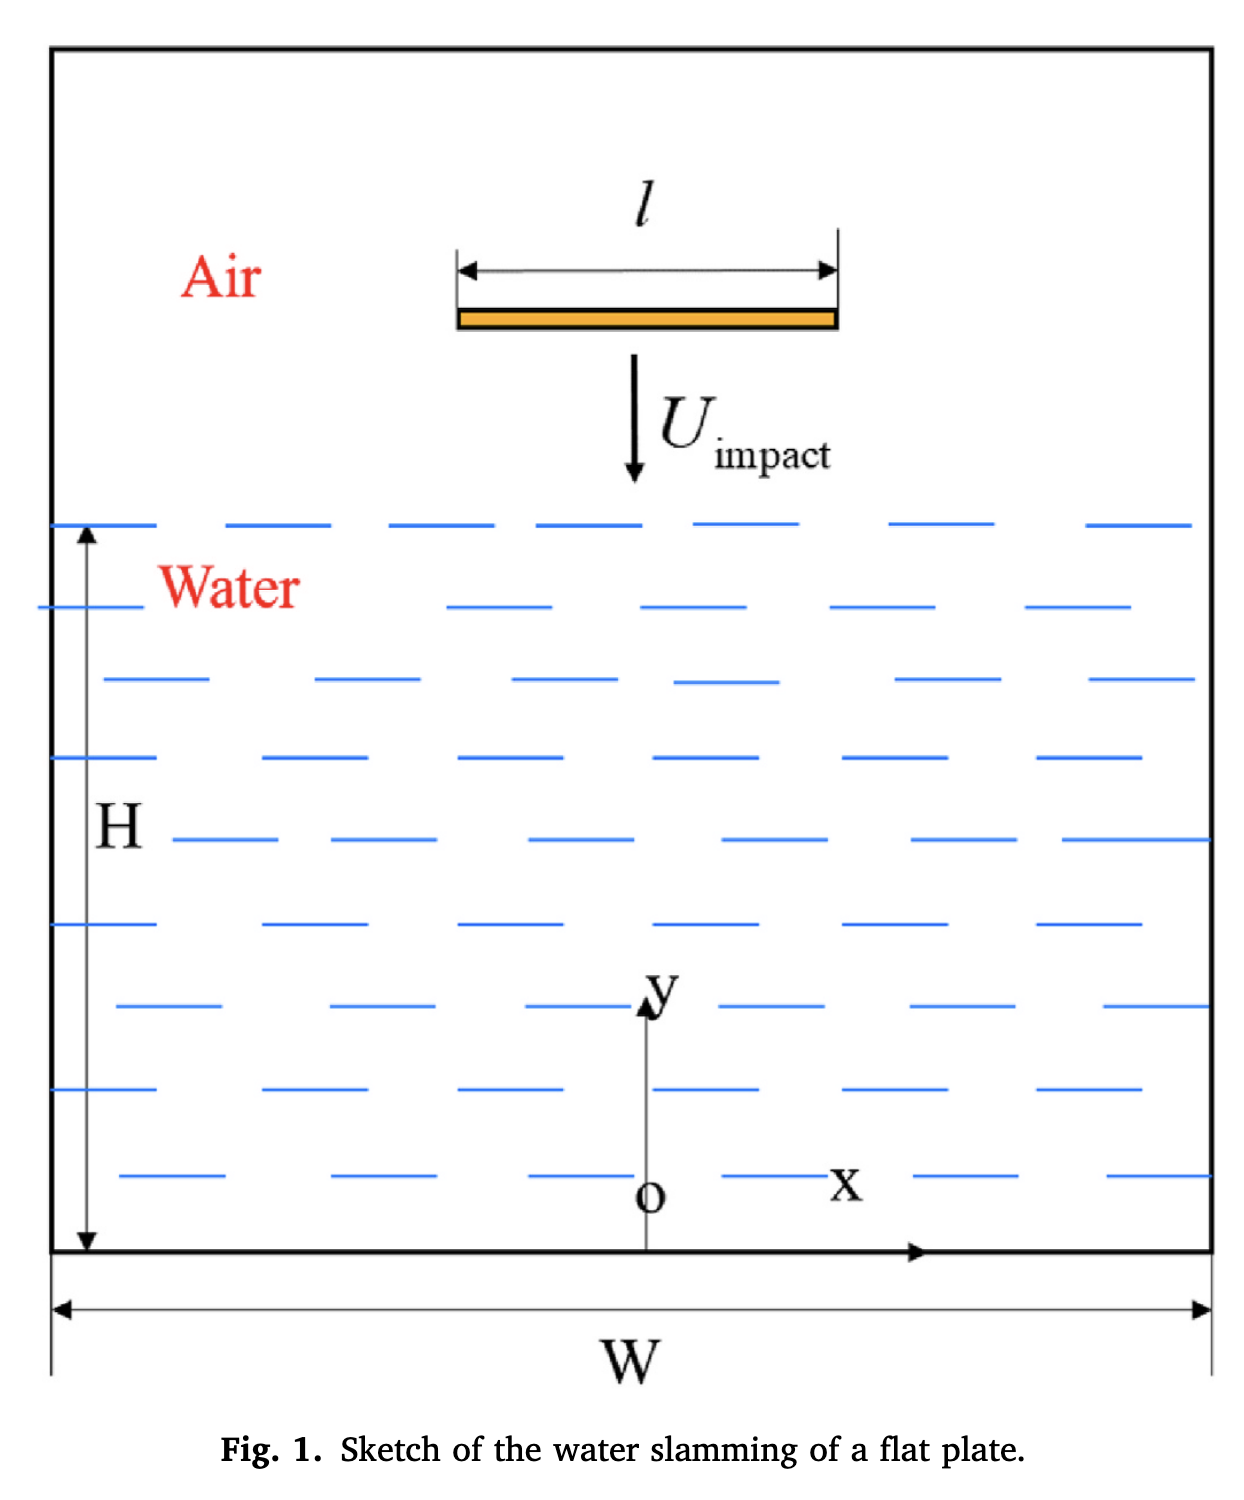
\includegraphics[width=30em]{./source/Fig1.png}
}
\paragraph{\quad}From the velocity field shown in Fig. 2, it can be observed that clear 
                circulating air jet surrounding the plate is generated during the falling process. 
                This is because the air under the plate is compressed during the falling of the 
                plate, causing the pressure of the air under the plate to increase and the pressure 
                of the air above the plate to decrease. As a result, the air flows around the edges 
                of the plate, which in turn forms a circulating air vortex as displayed in Fig. 2. 
                When the plate is about to contact with the water, the velocity of the air escaping 
                from both sides is very large even over $100 m/s$, although the impact velocity of the 
                plate is only$ 5.5 m/s $in this case. Similar situation can be found in the research of 
                Lind et al. (2015) in which it is believed that the high-speed subsonic flow is readily 
                formed for the air in the water slamming of plate even in a moderate impact event. 
                During the impact of plate, a part of air is trapped under the plate and forms the air 
                cushion for the slam plate, as shown in Fig. 3. At the same time, the pressure distribution 
                of the slam plate is displayed. Aiming at the numerical prediction of the slamming load 
                of the plate, the time histories of the pressure of the plate center and the slamming force 
                of the whole plate are given in Fig. 4 and Fig. 5, respectively. It can be found that 
                generally, the time history of the pressure at the center of plate obtained by adopted 
                the present SPH method agrees well with the FVM result provided by Ma et al. (2016) but a 
                little lower than the experimental data in (Ma et al., 2016). For the slamming force of 
                the whole plate, the present result obtains a higher peak compared with the SPH result of 
                Yang et al. (2020), and the result obtained by present SPH method shows good agreement 
                with the results of experiment and FVM method in Ma et al. (2016). In general, for the 
                present test of the water slamming of flat plate involving air-cushion effect, the present 
                method has good accuracy in predicting the slamming load of structure.
\paragraph{\quad}从速度场如Fig. 2,可以明显看出在下落过程中板周围产生了环状空气射流。这是因为板下空气在下落过程中被压缩,导致板下
            空气压力升高而板上空气压力下降。因此,空气绕过平板边缘流动,进而形成如Fig. 2所示的环状空气漩涡。尽管此时板的砰击速度只有$5.5m/s$
            当平板即将接触水面
            时,从板端逸出的空气速度非常大,甚至超过$100m/s$.类似的情况可以在Lind et al. (2015)的研究中发现,他认为对于空气而言在板与水的砰击过程中,
            即使在缓和的砰击情况下高速亚音速流也会快速形成。在板的砰击过程中,一部分空气困在板下并为砰击板形成缓冲,如Fig. 3所示。
            同时压力分布也如图所示。针对板的砰击载荷的预测,板中心压力的时间历程和整个板的砰击力分别由Fig. 4和Fig. 5给出。
            结果表明,由本文采用的SPH方法获得的板中心压力时间历程和由Ma et al. (2016)获得的FVM结果吻合的很好,但略低于
            (Ma et al.,2016)的实验数据。至于整个板的砰击力,本文的结果比Yang et al. (2020)的SPH结果的峰值更高,但
            本文SPH方法获得的结果和实验结果以及Ma et al.(2016)有很好的一致性。总而言之,对于包含气垫效应的平板和水的砰击实验,
            当前本文的方法表现出良好的结构物砰击载荷的预测精度。\\
{
    \centering
    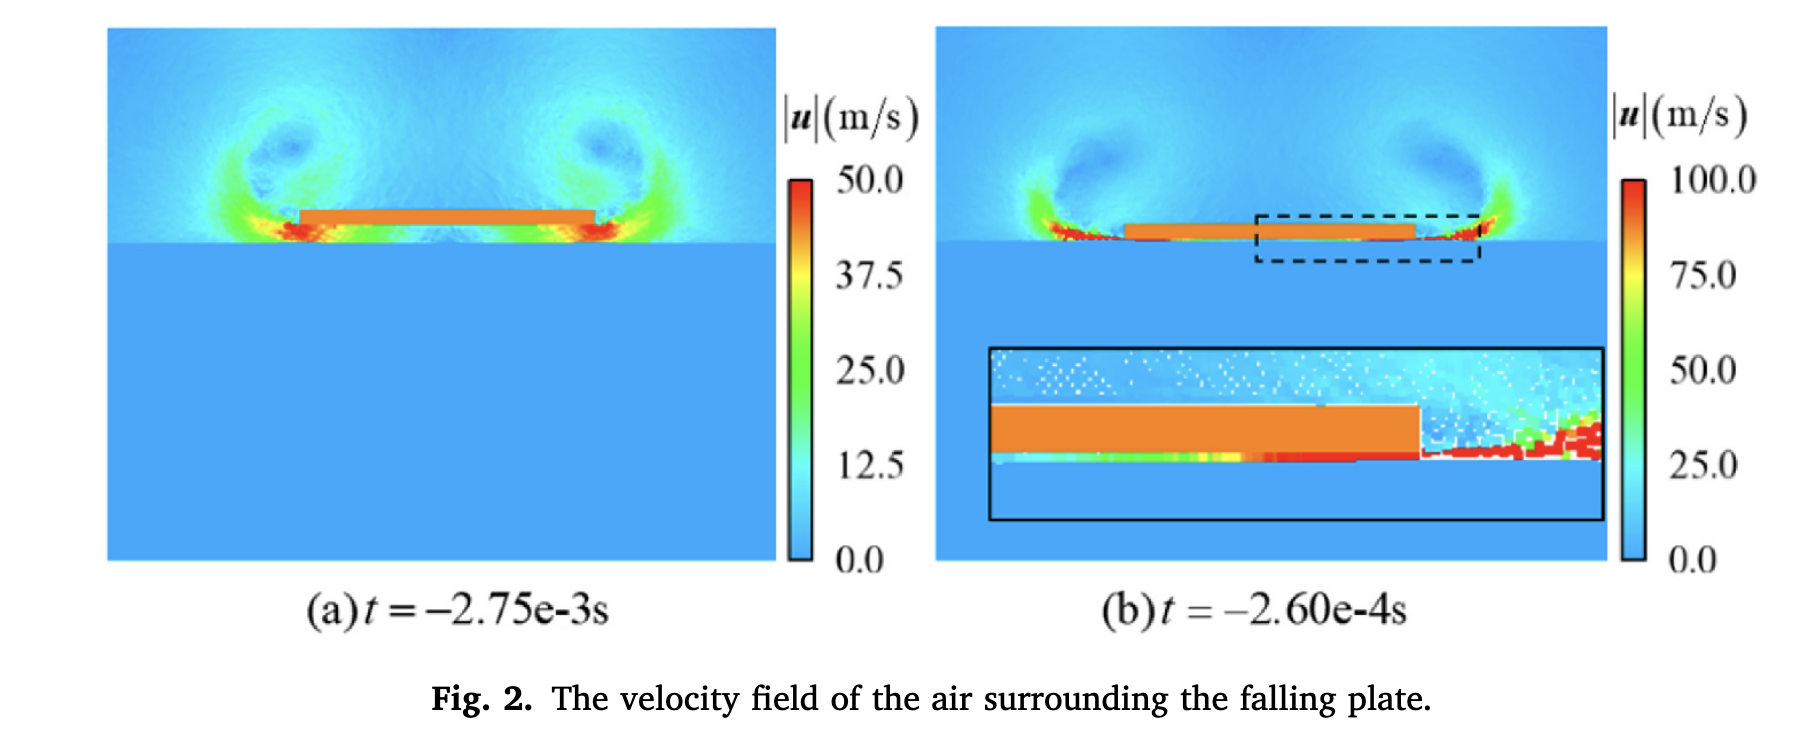
\includegraphics[width=30em]{./source/Fig2.png} \\
    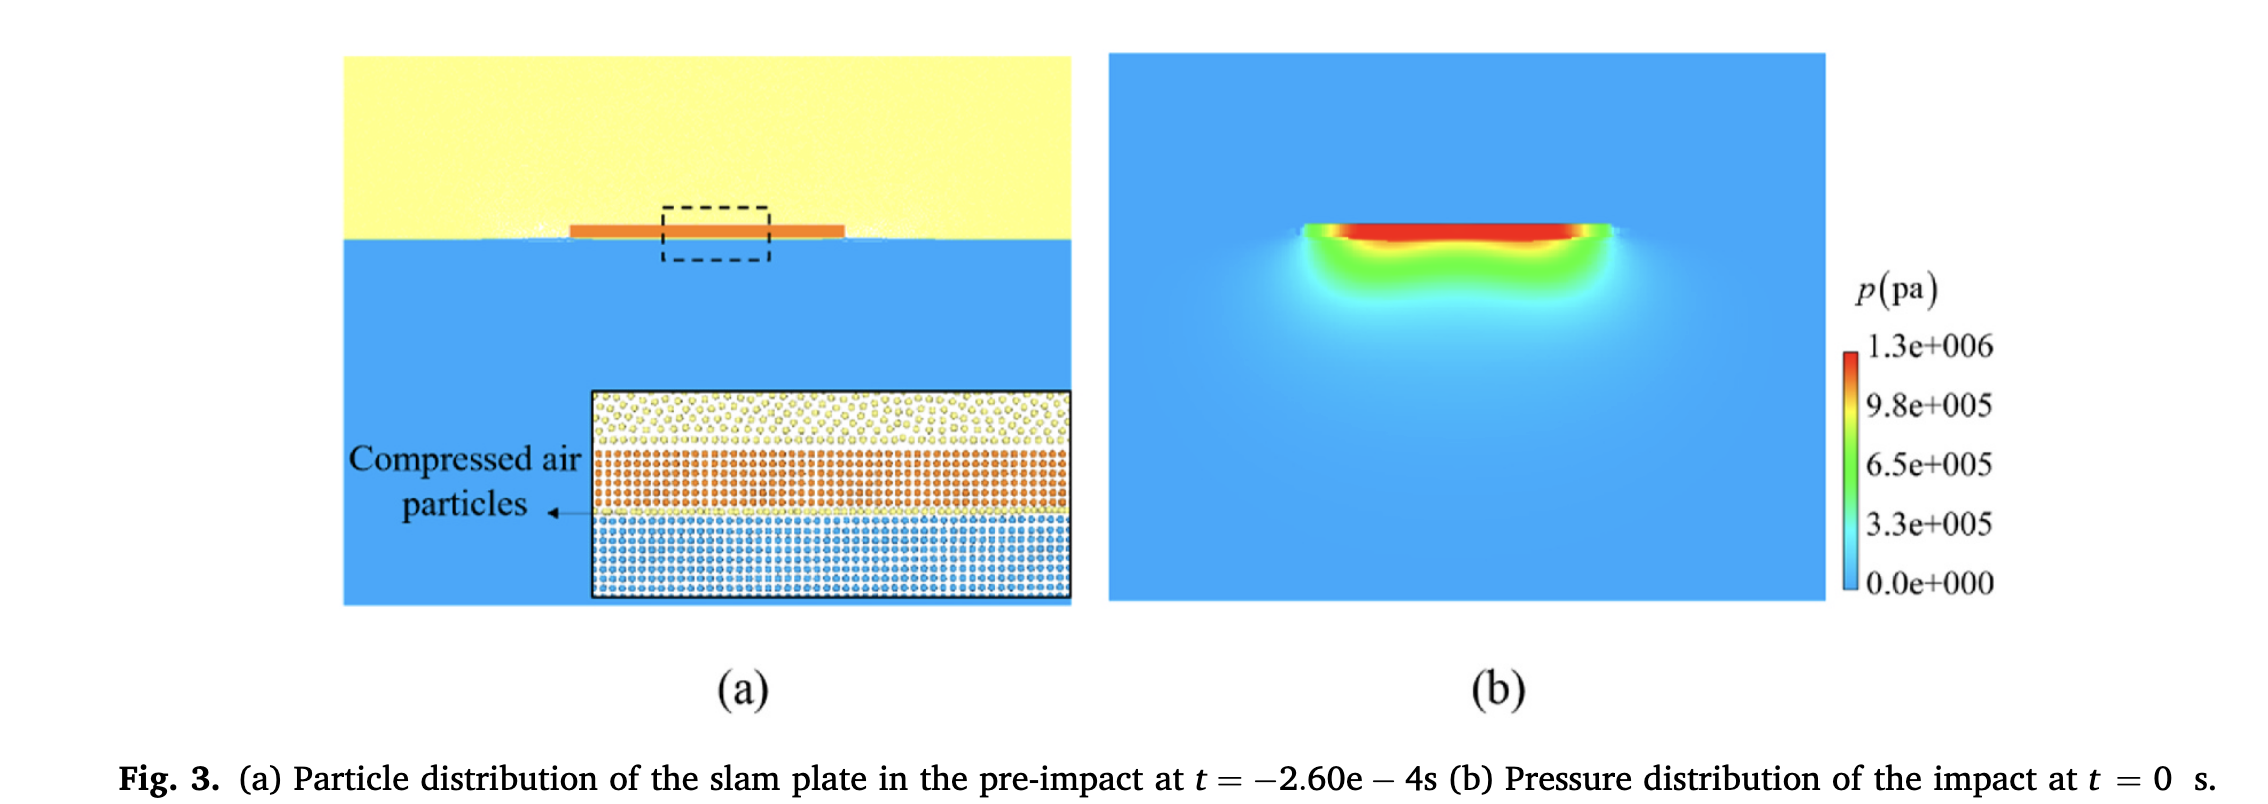
\includegraphics[width=30em]{./source/Fig3.png} \\
    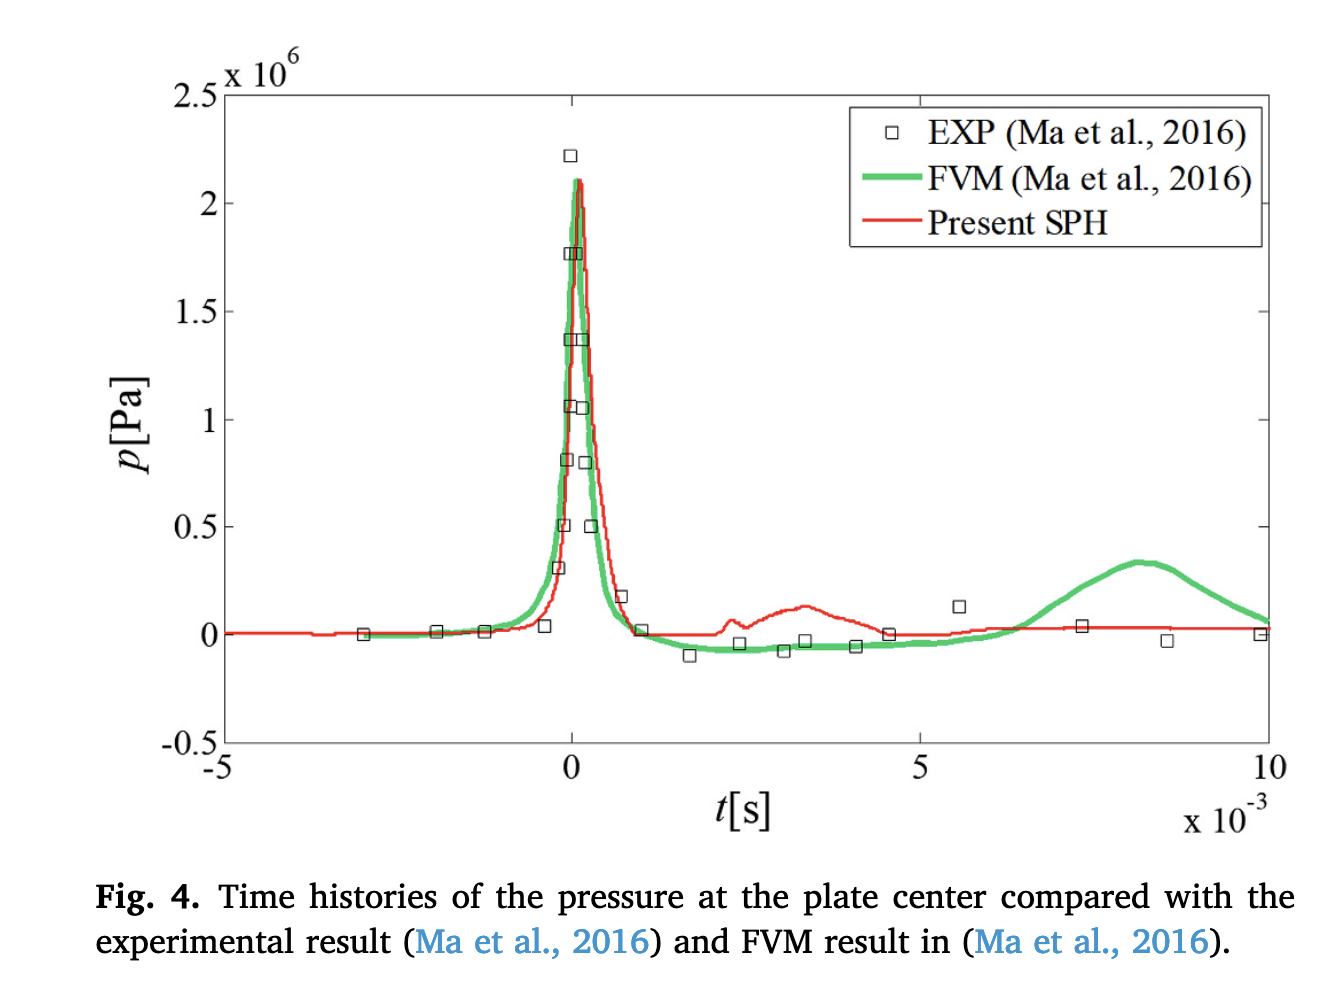
\includegraphics[width=30em]{./source/Fig4.png} \\
    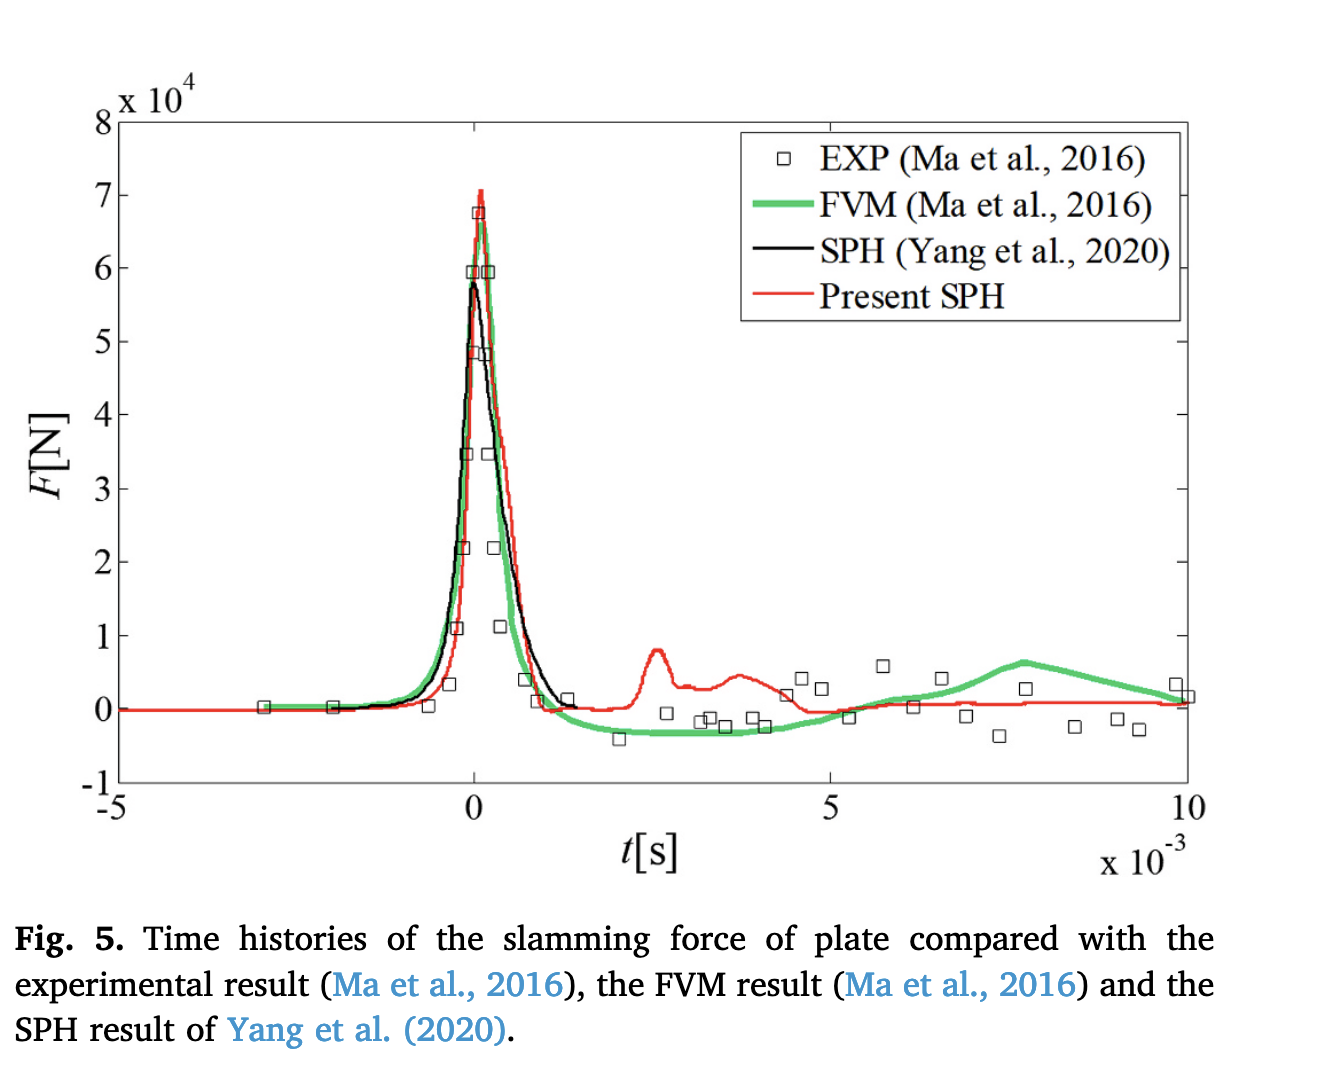
\includegraphics[width=30em]{./source/Fig5.png} \\
}

\paragraph{\quad}Furthermore, also through this numerical test, the convergence property of the 
                adopted SPH model is checked. Here, the simulations with the particle resolutions 
                of Δx = 0.003m and Δx = 0.0015m are performed, respectively. Combined with the 
                numerical results with Δx = 0.002m, the time histories of the pressure at the plate 
                center and the slamming force of whole plate with three different particle resolutions 
                are displayed in Fig. 6. It can be found that similar results of the pressure at the 
                plate center and the slamming load of plate are obtained with the particle resolution 
                increasing from Δx = 0.002m to Δx = 0.0015m, which indicates that the adopted SPH 
                scheme has a good convergence.
\paragraph{\quad}此外,此次数值试验验证了采用的SPH方法的收敛性质。这里分别进行了粒子分辨率为$\Delta x = 0.003m$
                和$\Delta x = 0.0015m$的模拟。结合$\Delta x = 0.002 m$的数值结果,不同粒子分辨率的板中心压力
                的时间历程和整个板的砰击压力如Fig. 6所示。可以发现粒子分辨率从$\Delta x = 0.002m$ 增加的$\Delta x = 0.0015m$
                时,板中心压力的时间历程和整个板的砰击力有类似的数值结果,这表明本文采用的SPH方法有良好的收敛性。\\
{
    \centering
    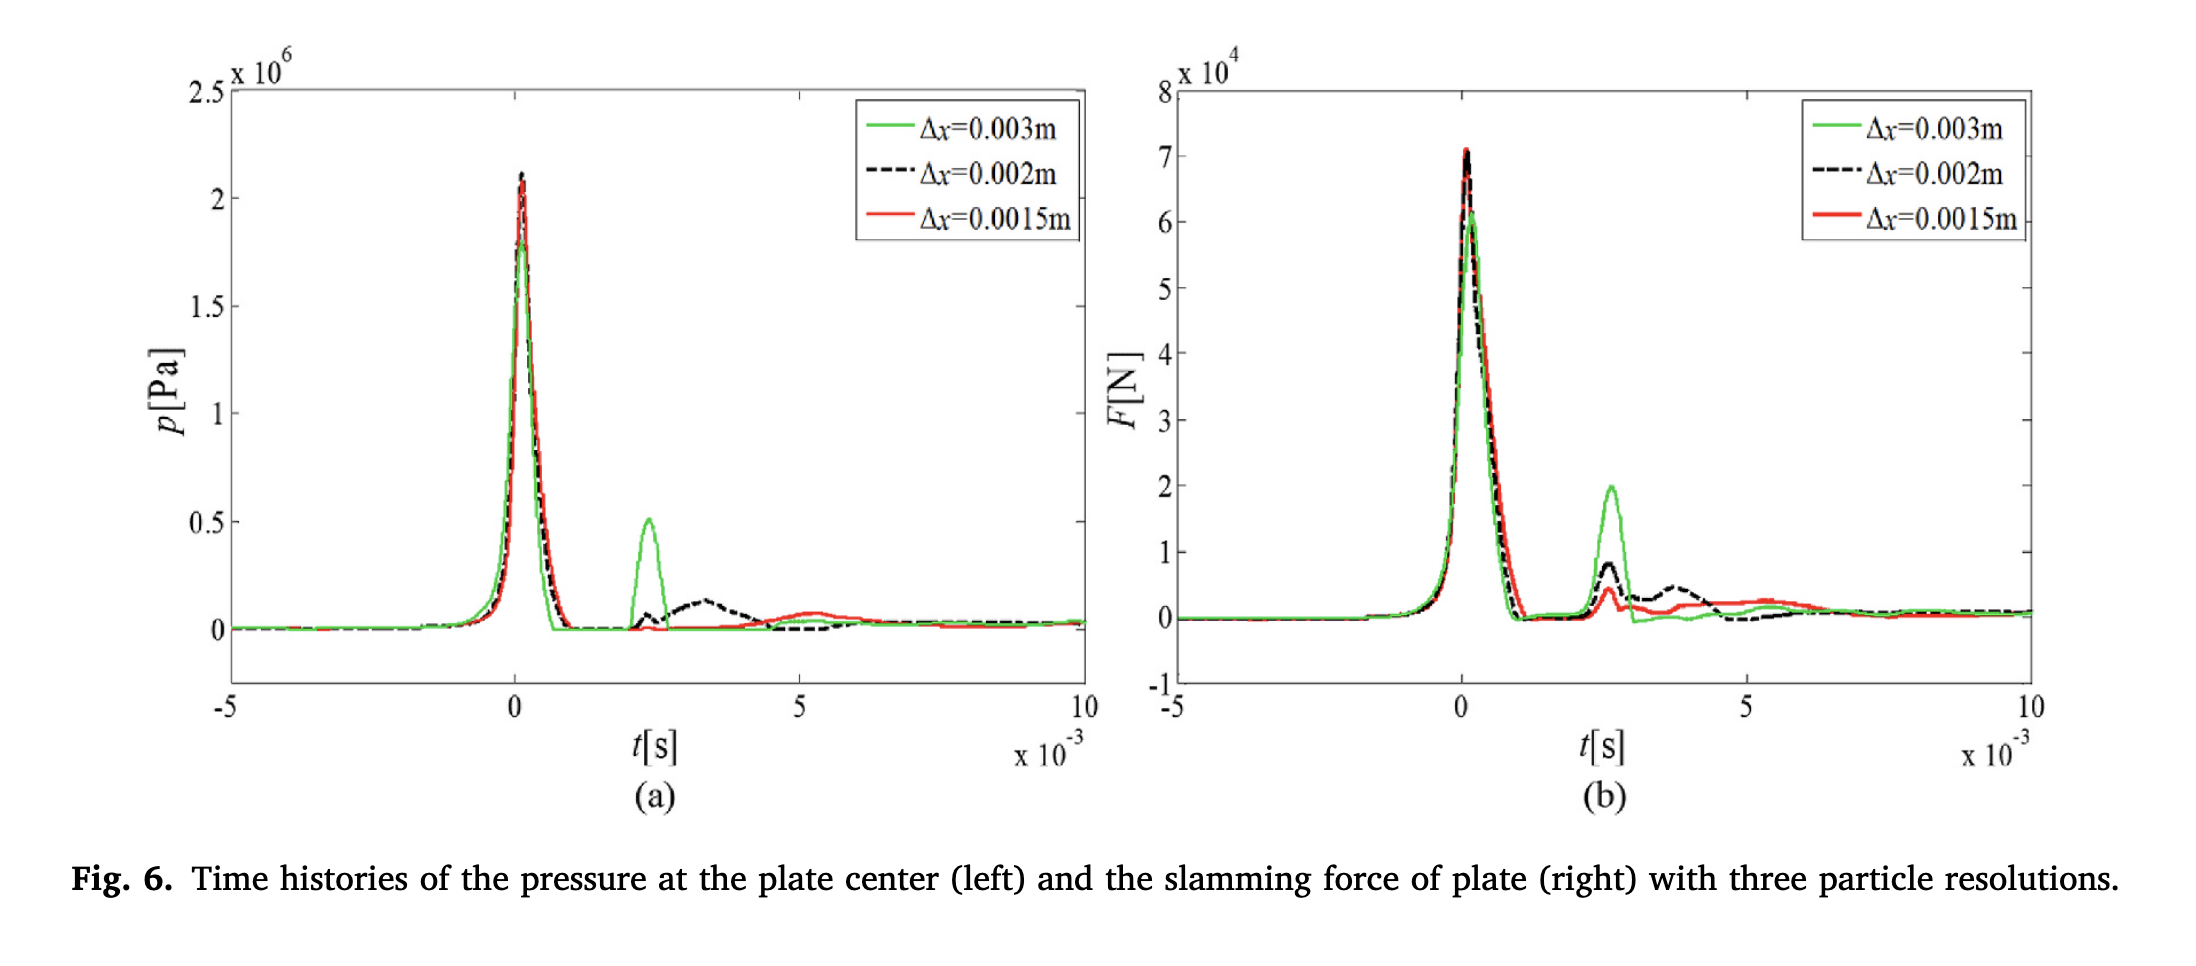
\includegraphics[width=30em]{./source/Fig6.png}
}
\subsubsection{Influence of the air on slamming load of flat plate-空气对砰击载荷的影响}
\paragraph{\quad}To investigate the effect of the air on the water impact of the flat plate, 
            the slamming loads of the plate obtained by taking the air into account or not are 
            compared. Fig. 7 shows the pressure distributions at$t = 0s$ of the computational 
            domain in the presence and absence of air, respectively. It can be seen that owing 
            to the existence of the air under the plate, the value of the slamming pressure of 
            the plate is reduced substantially, and the area of the pressure surface under the 
            plate is also reduced.
\paragraph{\quad}为研究空气对于平板和水砰击的效应,比较考虑和不考虑情况下的板的砰击载荷。Fig. 7分别展现了有空气和没有
                空气$t=0s$时计算域内的压力分布。结果表明,由于板底空气的存在,板的砰击压力的值大幅下降,而且板底
                的压力面面积也有所减小。\\
{
    \centering
    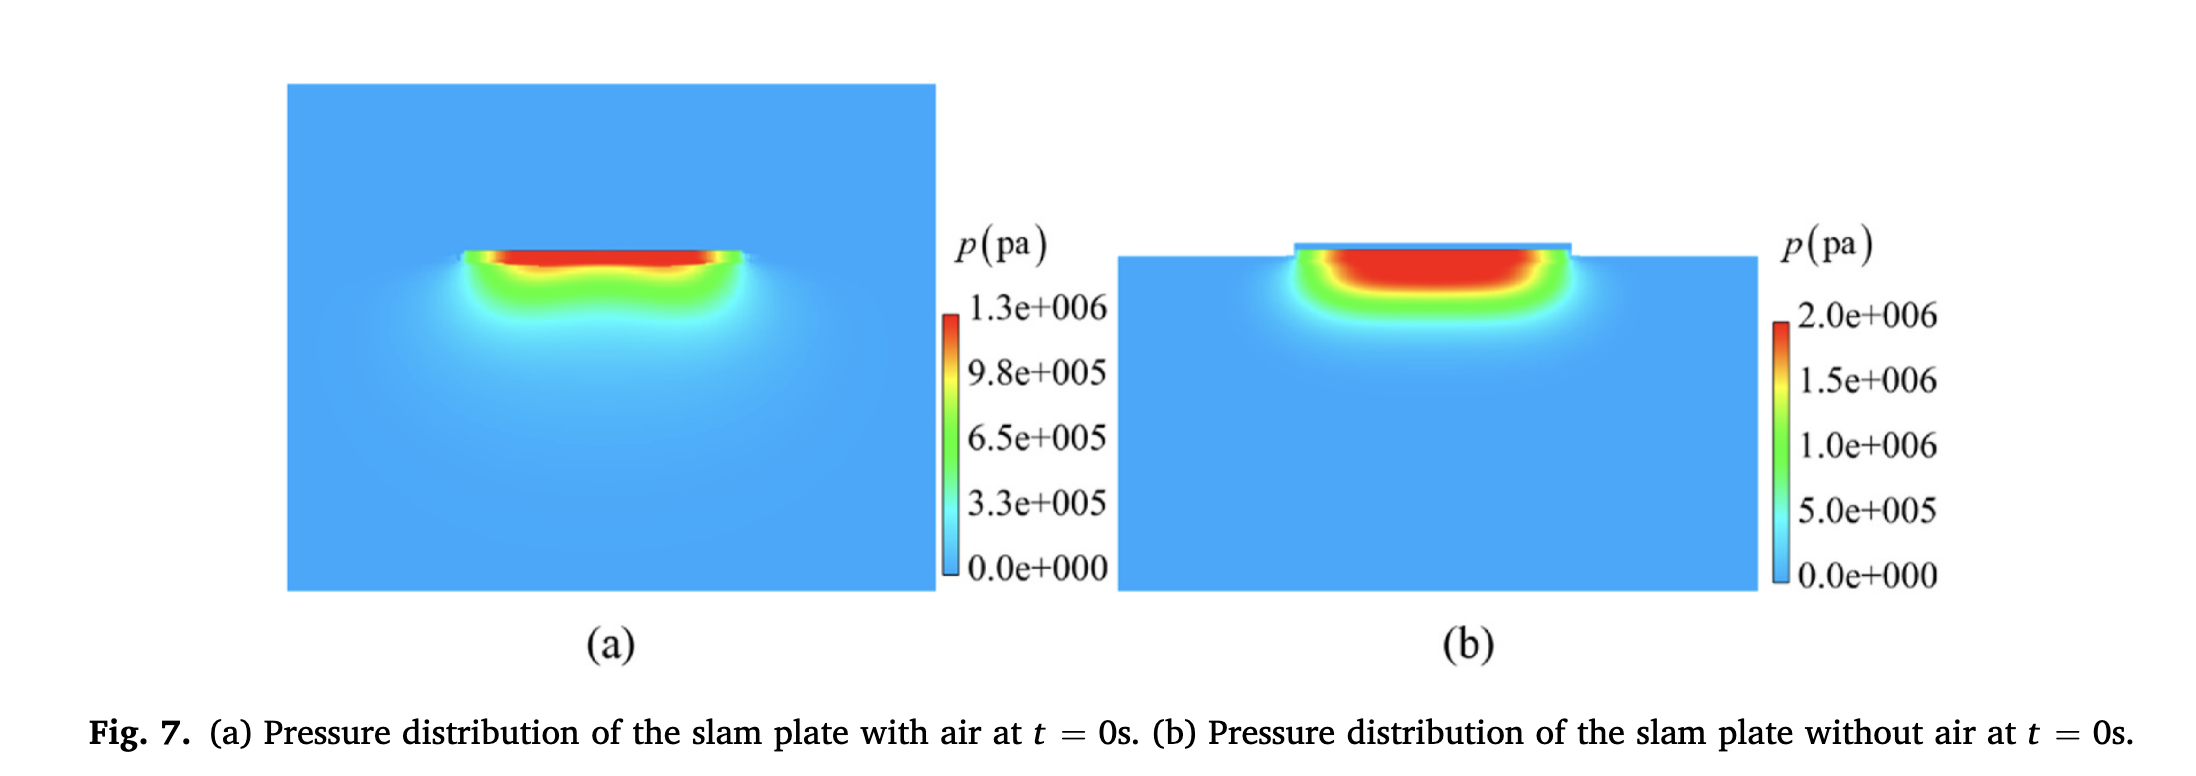
\includegraphics[width=30em]{./source/Fig7.png}
}

\paragraph{\quad}Fig. 8 displays the comparison of the slamming load of plate with and without air. 
                It can be seen that ignoring the air overestimates the magnitude of the slamming 
                load and underestimates the pulse width of the impact, which reflects the buffering 
                effect of air cushion for the impact. In addition, due to the existence of the air, 
                the reflection wave becomes obviously weakened in the post-impact. The reason is 
                that the impedance of the air is much smaller than that of the water. When the 
                reflected pressure wave propagates from the water to the air under the plate, 
                that is, from the high-impedance medium to the low-impedance medium, 
                the pressure wave is significantly reduced.
\paragraph{\quad}Fig. 8显示了有无空气的砰击载荷的比较。可以看书忽略空气导致过高估计了砰击载荷,却过低估计了砰击的宽度,
                其反应了气垫的缓冲效应。此外由于空气的存在,反射波在砰击后明显减弱。因为空气的阻抗远远小于水的阻抗。
                当反射压力波从水中传播到板下空气中时,即从高阻抗介质到低阻抗介质,压力波显著较小。\\
{
    \centering
    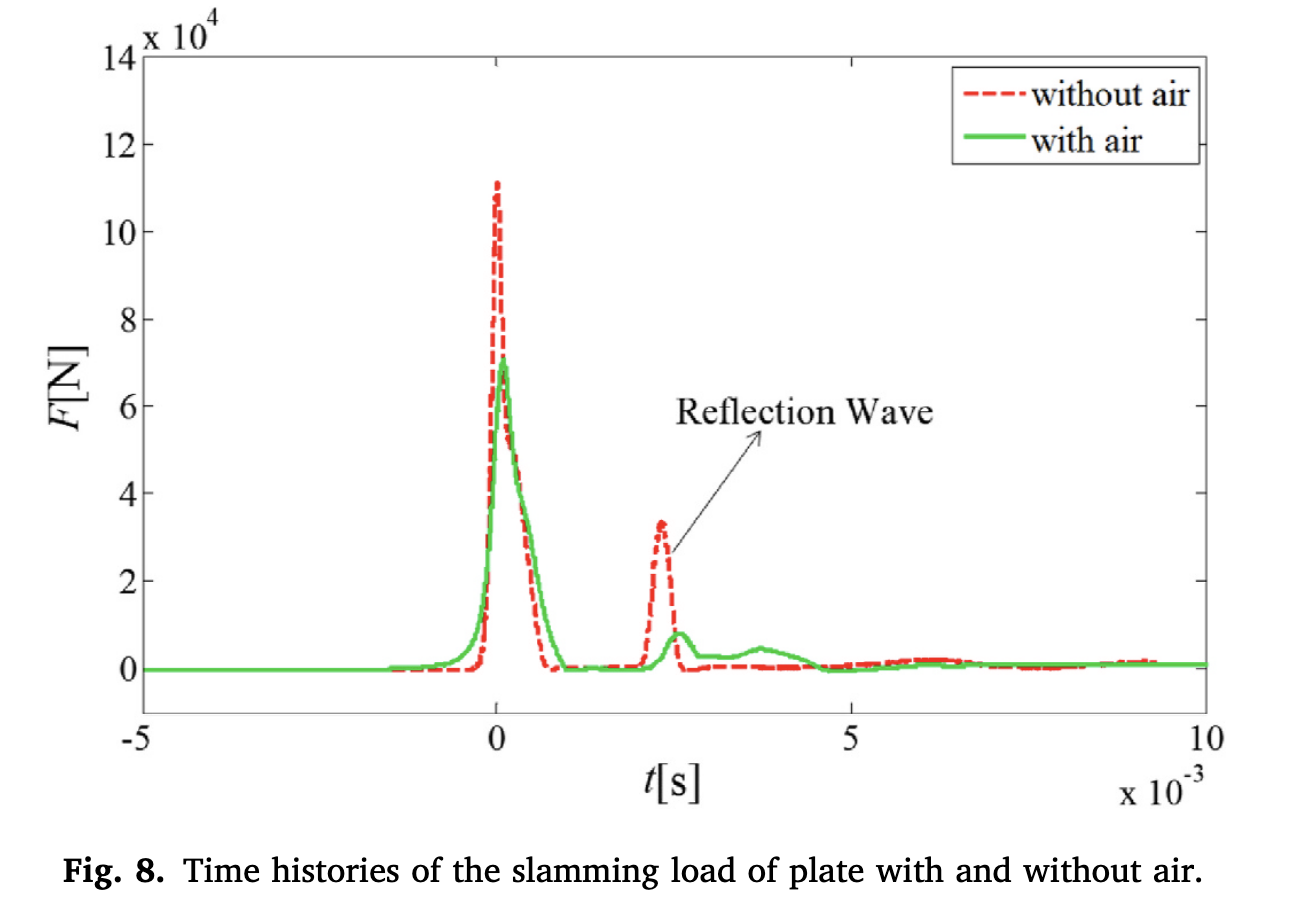
\includegraphics[width=30em]{./source/Fig8.png}
}
\subsubsection{Influence of the plate length on slamming load-板长对于砰击载荷的影响}
\paragraph{\quad}Fig. 9 shows the time histories of the slamming force of the plate 
                with different lengths in the presence and absence of air. It can be 
                found that the slamming force of the plate as well as the reflection 
                pressure load increase rapidly as the plate length becomes larger. 
                The reason accounts for this phenomenon is that a wider plate tends 
                to result in a larger contact area and thus a larger slamming load. 
                In addition, as shown in Fig. 9, ignoring the air obviously overestimates 
                the slamming load of the plate, and the buffering effect of the air cushion 
                becomes more significant with the increase of the plate length. More specifically, 
                in terms of the moment of water slamming, the change of plate length has little 
                influence on the contact time between the plate and water when the air is ignored. 
                However, when the air is taken into account, it is shown that with the increase of 
                the plate length, the occurrence time of the impact is delayed. The reason is that 
                the larger the plate length, the greater the amount of air trapped under the plate. 
                Therefore, under the compression effect of the air, the contact between the plate and 
                water becomes later, leading to the lag of the peak of the slamming load. From the 
                perspective of the magnitude of slamming load, Table 1 displays the comparison on 
                the peaks of the slamming force of plate with different lengths in the presence and 
                absence of air. Here, the peak values of the slamming force with and without air are 
                defined as $F_{air}$ and $F_{no_air}$, respectively. Owing to the more significant cushioning 
                effect of air under the wider plate, the difference in the peak value of the slamming 
                force in the presence and absence of air is getting larger, as shown in Table 1. 
                For the case with plate of $l = 0.5m$, the magnitude of the slamming force is reduced by 
                45.8\% thanks to the existence of the air.
\paragraph{\quad}Fig. 9展现了有无空气时不同板长的砰击压力的时间历程。可以发现随着板长增大,砰击载荷和反射压力载荷迅速增大。
                解释这一现象的原因是板长趋于越长,导致越大的接触面积,因而砰击载荷越大。此外,如Fig. 9所示,忽略空气会显著
                过高估计砰击压力,并且气垫的缓冲效应随着板长的增加变得更加显著。更具体而言,就入水砰击的时刻而言,当忽略空气时,
                板长的变化对空气和水的接触时刻影响很小。然而,当考虑空气时,结果表明随着板长增加,接触时刻会延后。其原因是
                当板长越长,困在板下的空气数目越多。因此,由于空气的压缩效应,板和水的接触变迟,导致砰击载荷峰值的滞后。从
                砰击载荷大小的角度看,Table 1比较了有无空气时不同板长的平板砰击力峰值。这里有无空气的砰击力分别用$F_{air}$和$F_{no_air}$
                表示。因为更宽的板下的缓冲效应更明显,有无空气的砰击力峰值的差异变得更大,如Table 1所示。在板长$l = 0.5m$的情况下,
                得益于空气的存在,砰击力的大小减小了45.8\%。\\
{
    \centering
    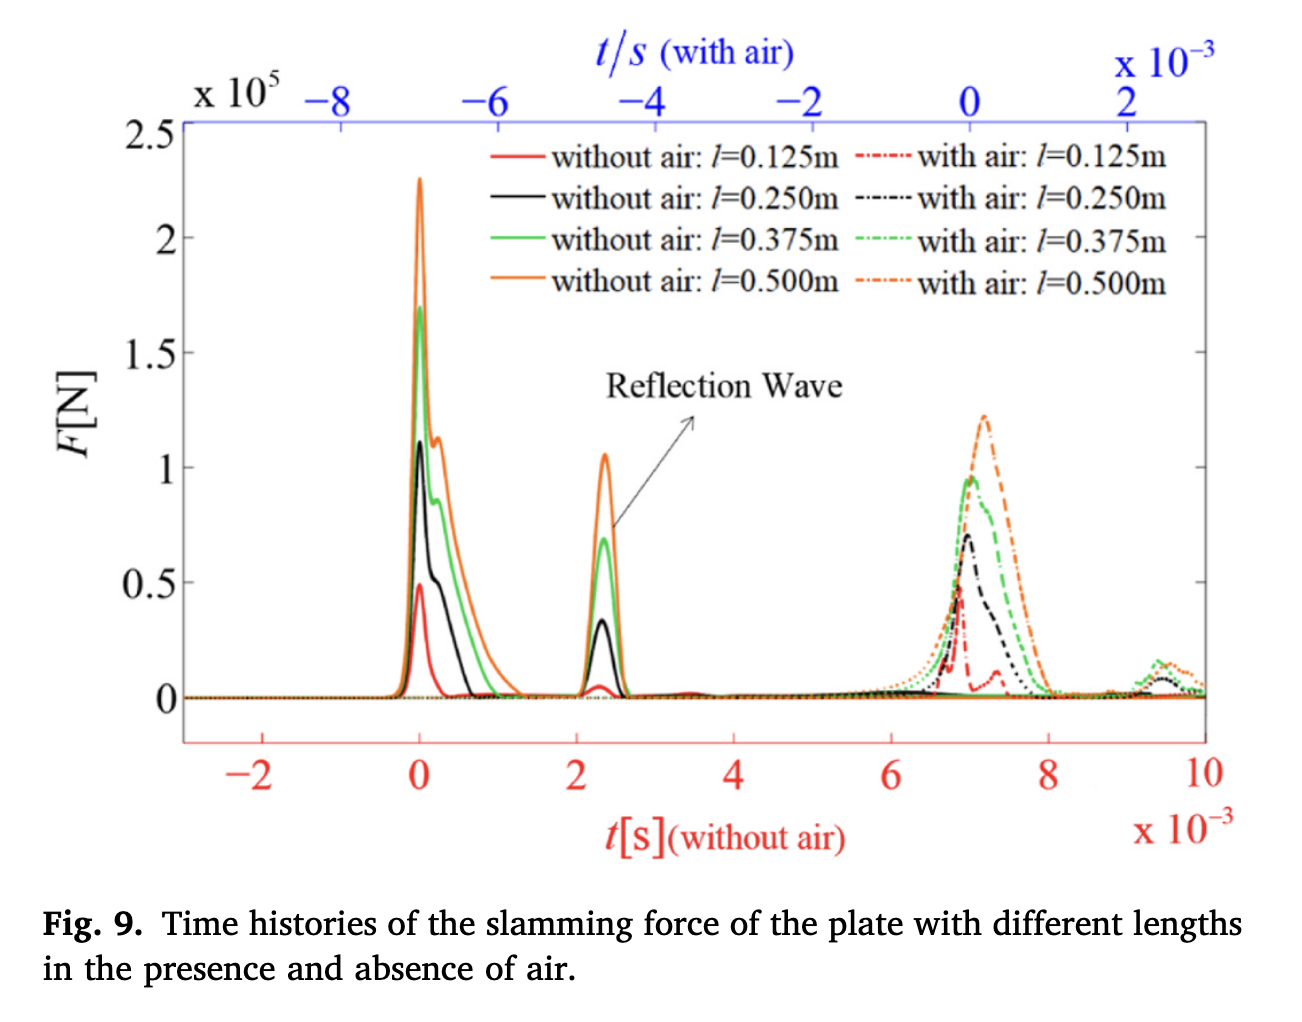
\includegraphics[width=30em]{./source/Fig9.png}
}

\subsection{Slamming of LNG tank insulation panel-LNG船绝缘板砰击}
\subsubsection{Simulation of slamming process}
\paragraph{\quad}In this subsection, focusing on the air-cushion effect in the water entry, 
                a complex practical problem studied in Marrone et al. (2017), i.e., the slamming 
                of the LNG tank insulation panel, is simulated, and the related accuracy test is 
                provided in Appendix A. For the simulation of the slamming of LNG tank insulation 
                panel in the present work, the computational model including the water region and 
                the insulation panel is sketched in Fig. 10, which is similar to that in Marrone 
                et al. (2017). In the present simulation, the mass of the insulation panel is $69.7 kg$, 
                and the insulation panel impacts on the water with a vertical velocity of $5.5 m/s$. 
                The particle resolution is set to $\Delta x = 0.002m$, and the whole computational domain 
                is discretized into 312992 particles.
\paragraph{\quad}在本小节中,模拟了Marrone et al. (2017)研究的一个复杂的工程问题,即LNG船绝缘板的砰击,重点研究了
                入水过程中的气垫效应,并在附录A中提供相应的精度测试。对于本文的LNG船绝缘板的模拟,计算模型与Marrone et al. (2017)
                类似,包括水域和绝缘板,如Fig. 10所示。本文的模拟中,绝缘板的质量时$69.7Kg$,绝缘板的与水砰击的速度是
                $5.5m/s$。粒子分辨率设置为$\Delta x = 0.002m$,整个计算域离散为312992个粒子。\\
{
    \centering
    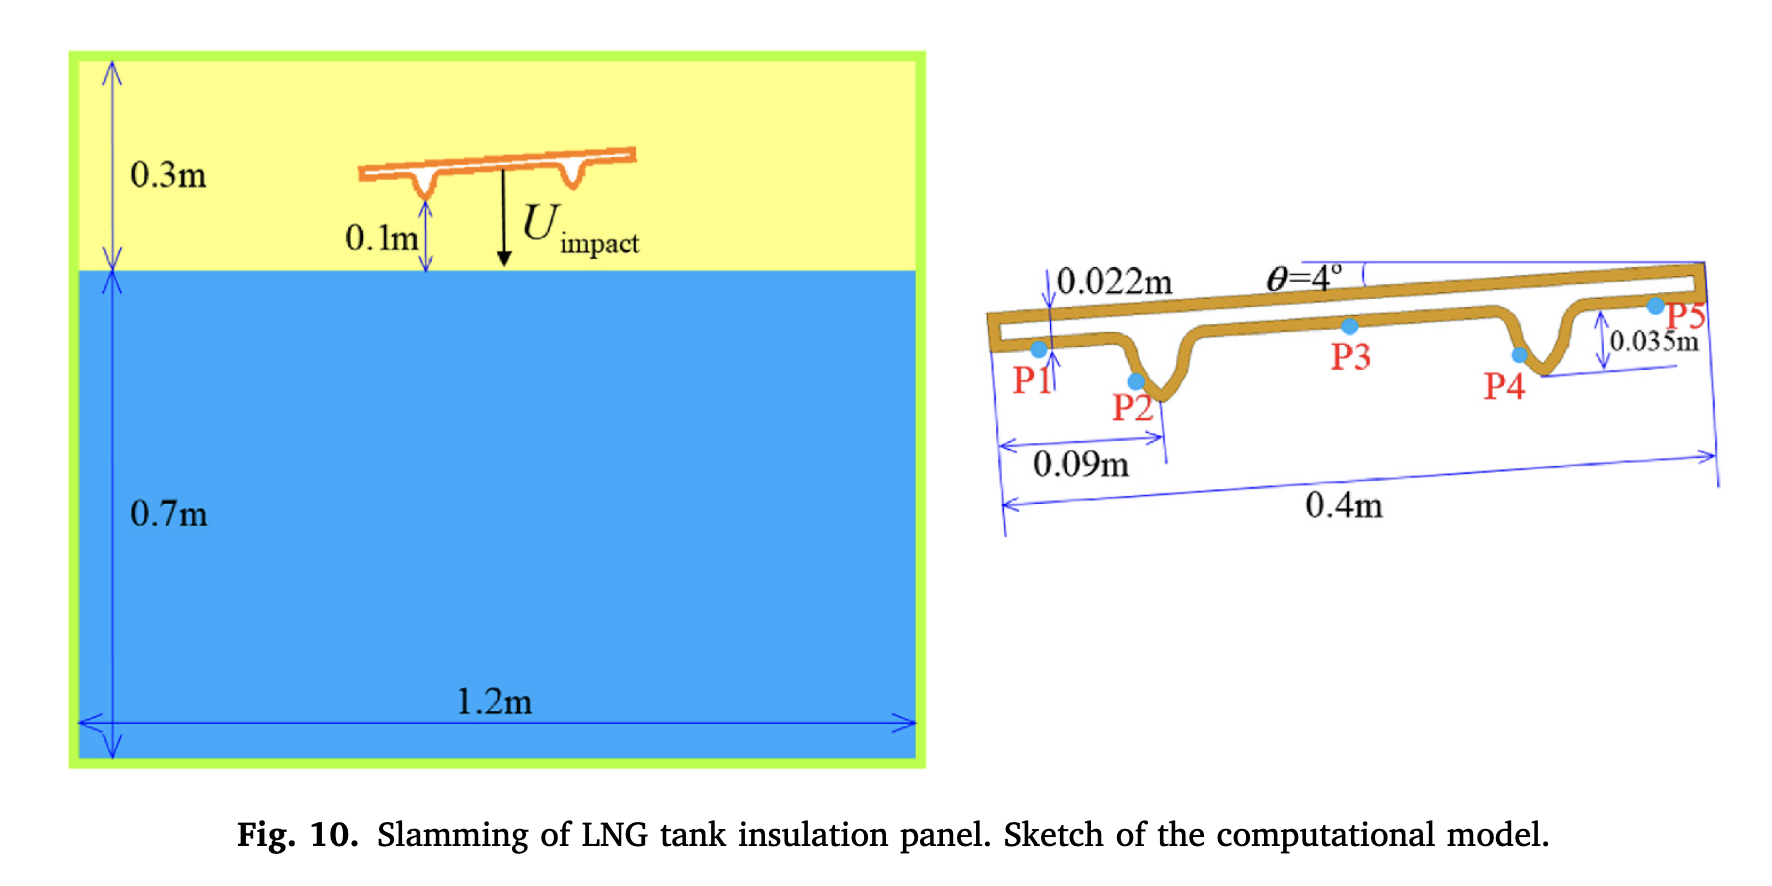
\includegraphics[width=30em]{./source/Fig10.png}
}
\paragraph{\quad}Fig. 11 shows the particle distributions and corresponding pressure 
                fields at several typical time instants. It can be seen that with the 
                fall of the panel, the left dent of the plate first touches the water 
                surface at about t = 0.0186s. Subsequently, the right dent impacts on 
                the water, and an air bubble is generated by the entrapment of the air. 
                During $t \in (0.0207s, 0.0237s)$, as the panel continues to fall, the bubble 
                volume decreases and thus the bubble pressure increases. It can be seen 
                that the pressure inside the bubble is uniform and continuous across the 
                waterair interface. At t = 0.0237s, the left corner of the panel impacts 
                on the water violently, producing a large impact pressure wave. At last, 
                the right corner of panel impacts on the water with the impact pressure 
                peak much smaller than that produced by the impact of the left corner. 
                During $t \in (0.0237s, 0.0282s)$, the air bubble expands and overflows from 
                the right dent, and because of the increase of volume of the air bubble, 
                the bubble pressure becomes lower.
\paragraph{\quad}Fig. 11给出了几个典型时刻的粒子分布和相应的压力场。可以看出随着平板的下落,左齿大约在$t=0.0186s$首先
                接触水面。随后,右齿与水砰击,并且由于空气的卷入产生了气泡。在$t \in (0.0207s,0.0237s)$
                时间内,随着板持续下落,气泡的体积减小而气泡内压力上升。可以看出,气泡内部的压力在整个
                水气界面处是均匀且连续的。在$t=0.0237s$时,板的左角与水面猛烈砰击,产生了巨大的砰击压力波。
                最后,板的右角与水面砰击,其砰击压力波峰值远小于右角砰击所产生的。在$t \in (0.0237s,0.0282s)$时间内,
                气泡膨胀并从左齿逸出,由于气泡体积的增大,其压力开始减小。\\
{
    \centering
    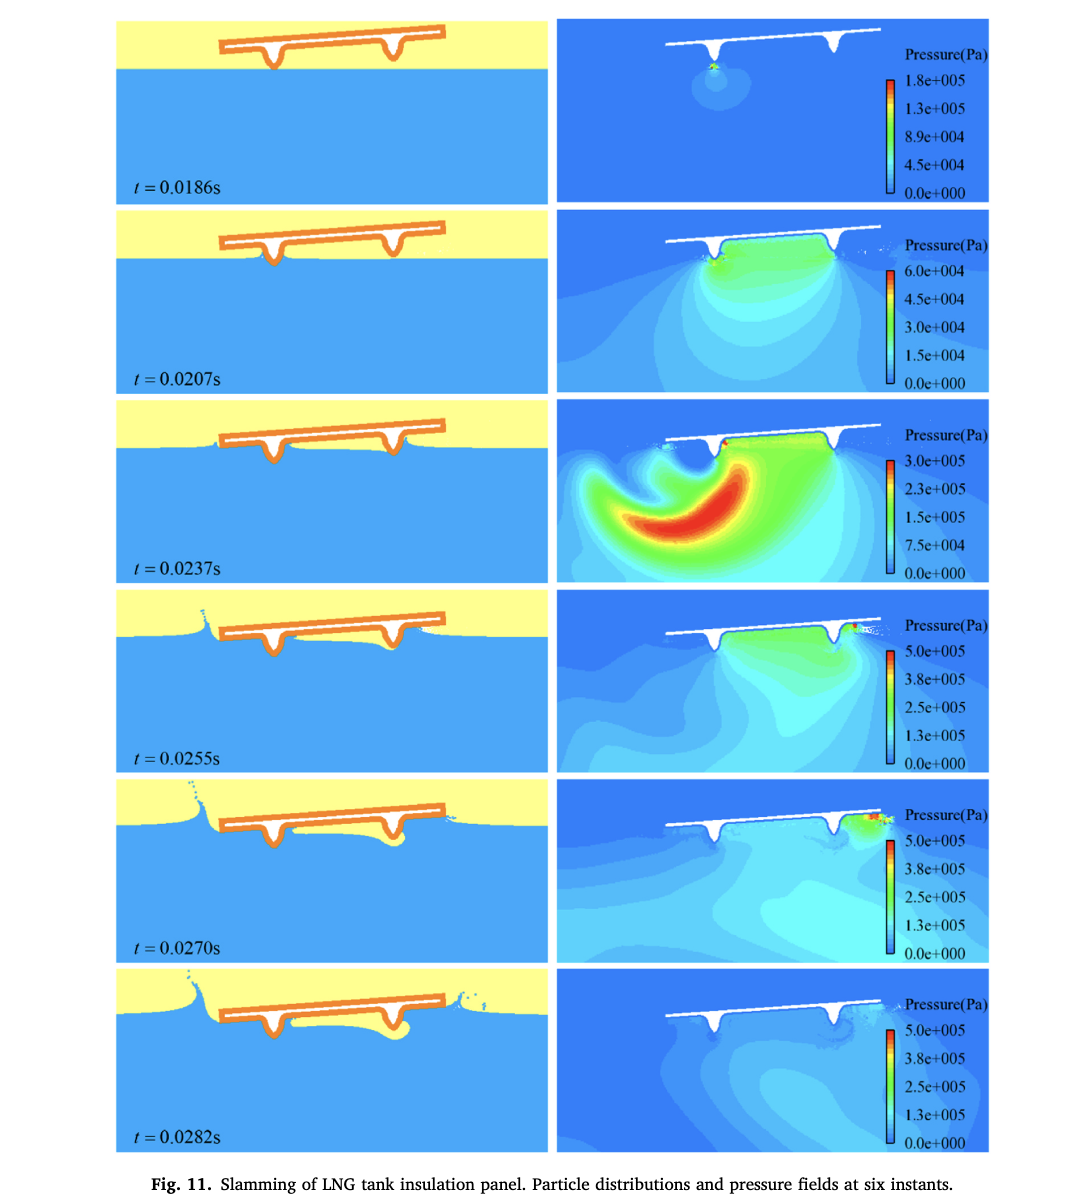
\includegraphics[width=30em]{./source/Fig11.png}
}
\paragraph{\quad}Fig. 12 gives the time histories of the pressure of the five measuring 
                points on the panel. It can be observed that for the point P1 which is 
                located at the left corner of the panel, its pressure peak is the largest 
                among all the measuring points. This large pressure load results from the 
                slamming by the high-speed water jet generated near the left dent. 
                For P2 which is on the left side of the left dent, although this measuring 
                point contacts with water earliest, the pressure peak is much smaller than 
                that of P1. The reason is that the water impact occurs at a certain angle 
                for P2, which considerably reduces the slamming load. Different from the 
                other measuring points, the pressure histories curves of P3 and P4 are very 
                smooth without obvious oscillations, and their peak values are closed but 
                much smaller than those of other measuring points. This can be explained by 
                the fact that these two points are surrounded by the air bubble entrapped by 
                the panel during slamming, so their pressure is approximately equal to that of 
                the air-bubble, and the slamming load is reduced significantly due to the buffering 
                effect of the air-cushion. For P5, its pressure peak becomes oscillatory again due 
                to the absence of aircushion. Besides, because of the decrease of the velocity 
                of the panel, the peak value of P5 is less than that of P1.
\paragraph{\quad}Fig. 12给出了板上五个测量点压力的时间历程。可以看出板的左角的P1点的压力峰值是所有测量点中最大的。
                这个大压力载荷是由左齿附近的高速水射流砰击造成的。P2位于左齿的左侧,尽管该测量点最先接触水面,但是其
                压力峰值远小于P1的。原因是与水对P2的砰击发生在的某个特定的角度,从而大幅地减小了砰击载荷。
                与其他测量点不同,P3和P4的压力曲线非常平滑,没有明显的震荡,而且它们的峰值非常接近,但远小于其他测量点的峰值。
                这可以被解释为事实上这两个点被板下落过程中困住的气泡所包围,所以其压力与气泡压力近似相等,
                并且由于气垫的缓冲效应,砰击载荷大幅降低。对于P5,由于气垫的消失,其压力再次出现震荡。此外,由于板的速度的下降,
                P5的峰值也小于P1.\\
{
    \centering
    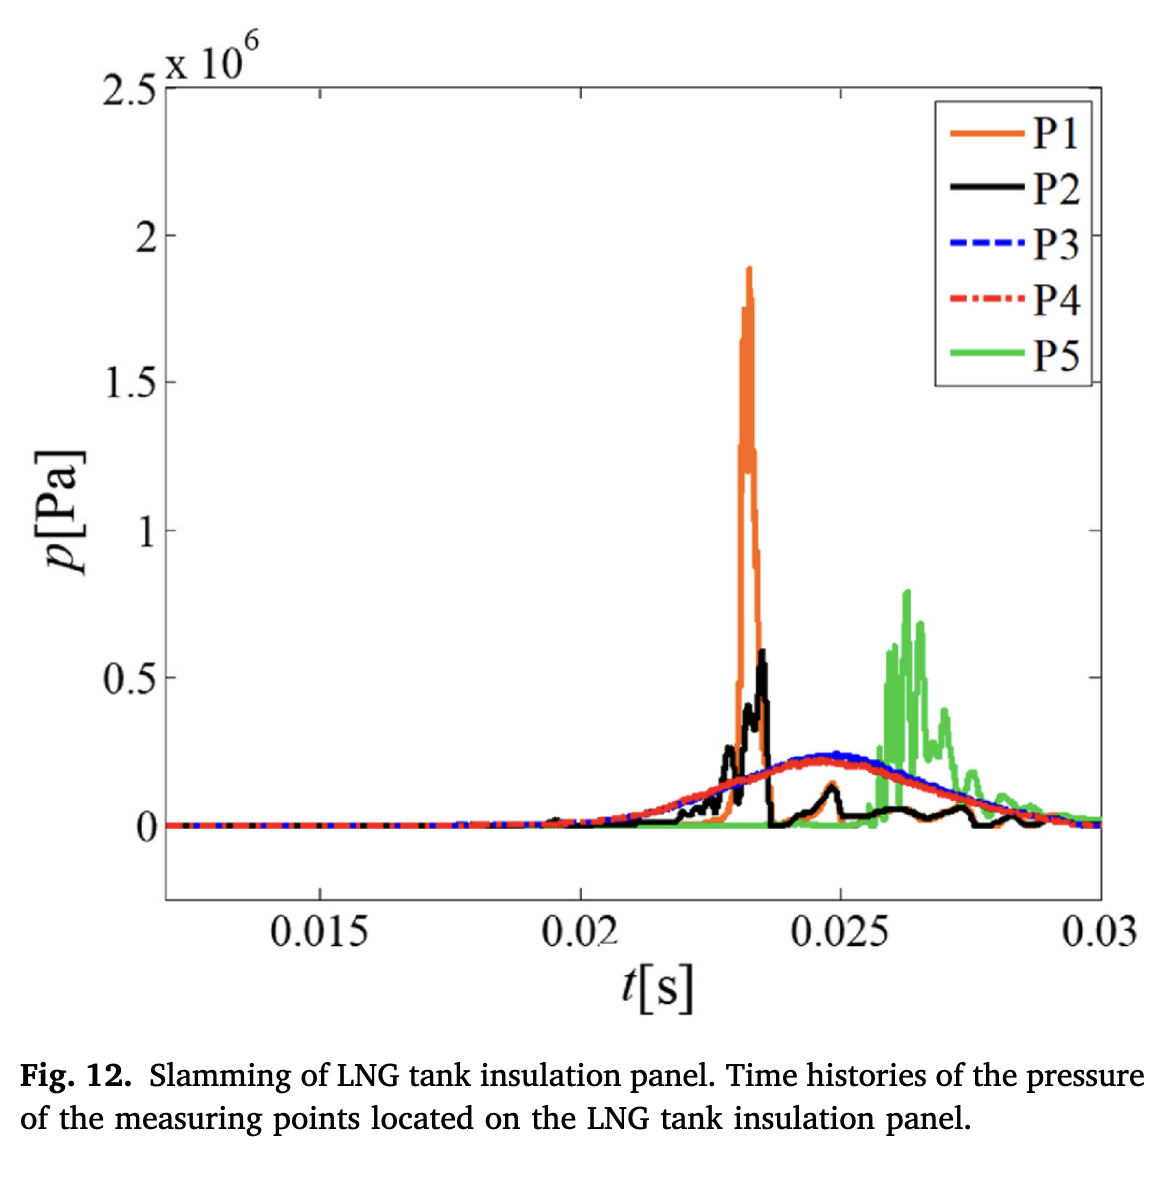
\includegraphics[width=30em]{./source/Fig12.png}
}
\subsubsection{Influence of the impact velocity on slamming of LNG tank insulation panel-砰击速度对于LNG船绝缘板砰击的影响}
\paragraph{\quad}To investigate the effect of impact velocity on slamming pressure of LNG tank insulation panel, the 
                simulations are conducted by adjusting the initial impact velocity to $\mathbf{U}_{impact} = 2.5m/s$ and 
                $U_{impact} = 4m/s$, respectively, and other conditions are same as those in subsection 3.2.1. 
                Combined with the obtained numerical result with $\mathbf{U}_{impact} = 5.5m/s$, the influence of impact 
                velocity on load characteristics at different measuring points on the panel is discussed. 
                Fig. 13 displays the particle distributions of the water slamming of LNG tank insulation 
                panel with different impact velocities. It can be observed that when the impact velocity 
                ranges from 2.5m/s to 5.5m/s, the evolution of the water surface and the air-cushion are similar. 
                When the impact velocity increases, the splash caused by the slamming becomes more intense and the 
                volume of the generated air bubble under the panel is smaller. To investigate the effect of impact 
                velocity on the slamming load of LNG tank insulation panel, Fig. 14 gives the time histories of the 
                pressure of the five measuring points on the panel with different impact velocities. Because the panel 
                with lower velocity falls in air for a longer time, the pressure peak of measuring points at the panel 
                with lower velocity appears later, but the trends of the time histories of the pressure of the measuring 
                points are also similar. Further, for all measuring points, the slamming pressure peaks increase 
                monotonously with the increase of slamming speed. For all the three cases with different impact 
                velocities, the maximum slamming loads are all recorded at the measuring point P1, and the three 
                pressure peaks are 1.88 MPa, 1.49 MPa and 0.61 MPa, respectively.
\paragraph{\quad}为了研究砰击速度对于LNG船保温杯砰击压力的影响,分别调整初始砰击速度为 $\mathbf{U}_{impact} = 2.5m/s$和 
                $U_{impact} = 4m/s$,其他条件和subsection 3.2.1相同,并进行模拟。结合已获得的 $\mathbf{U}_{impact} = 5.5m/s$数值
                结果,讨论了砰击速度对于不同测量点的载荷特性。Fig. 13给出了不同速度的LNG船绝缘板与水砰击的粒子分布情况。
                可以看到砰击速度从2.5m/s到5.5m/s,水面和气垫的演变类似。当砰击速度增加,砰击造成的飞溅更加剧烈并且板底生成气泡的体积更小。
                为了研究砰击速度对于LNG船保温杯砰击压力的效应,Fig. 14给出了不同砰击速度下板上五个测量点的压力时间历程。因为速度越低
                的板在空中下落时间更长,所以更低速度的板的压力峰值出现地更晚,但是测量点压力随时间变化的趋势相似。
                此外,所有测量点的压力峰值随着砰击速度的增加而单调增加。在不同砰击速度的三种情况下,最大砰击载荷都记录在测量点P1,并且三个
                压力峰值分别为1.88MPa,1.49MPa和0.61MPa.\\
{
    \centering
    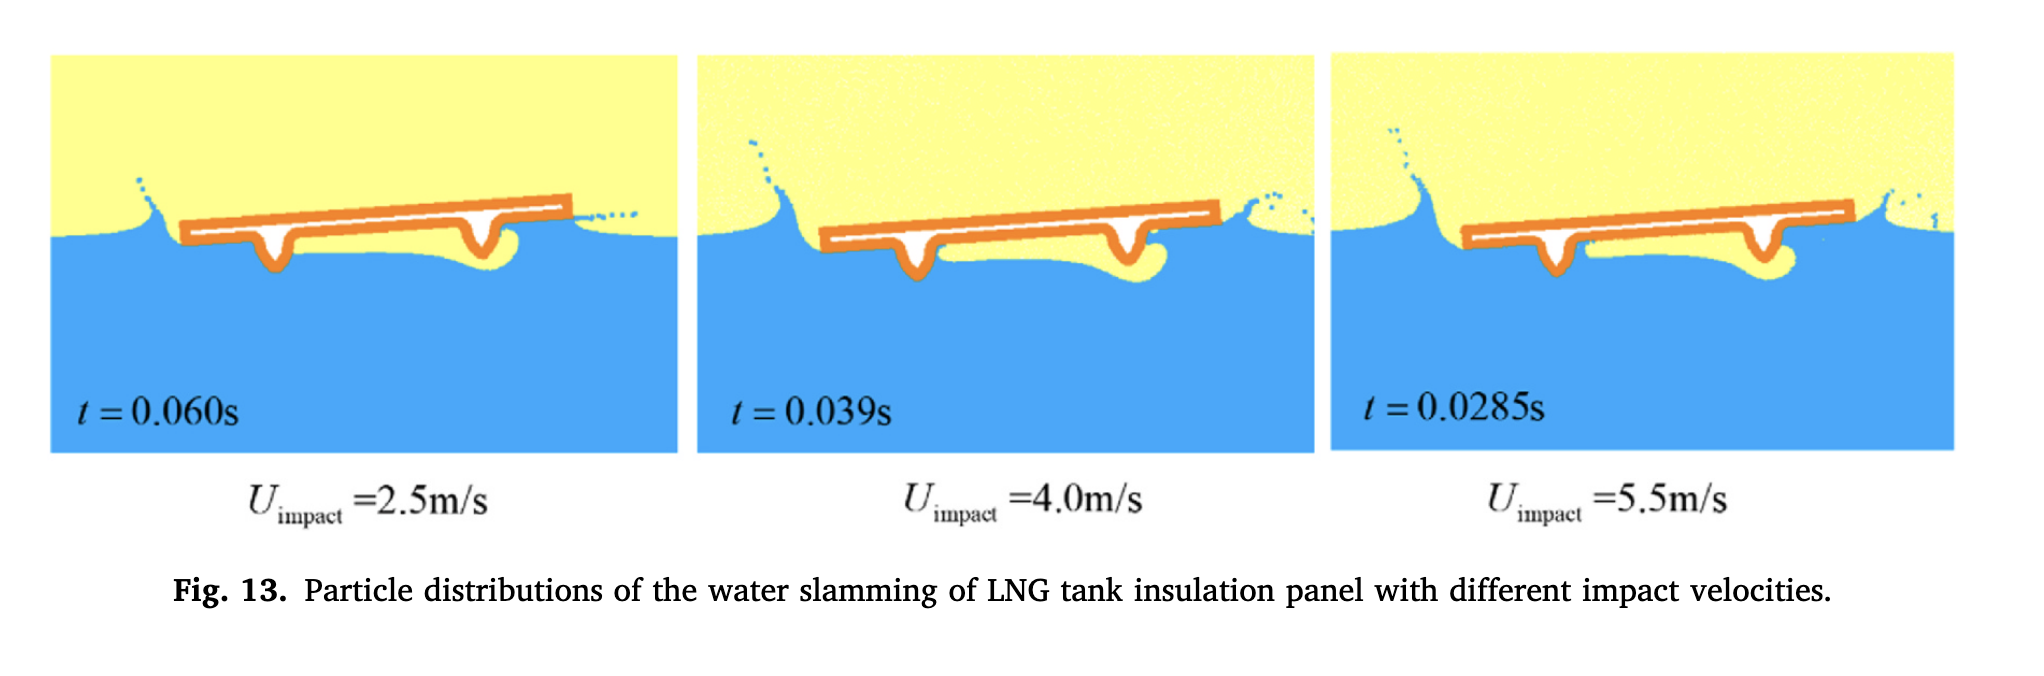
\includegraphics[width=30em]{./source/Fig13.png} \\
    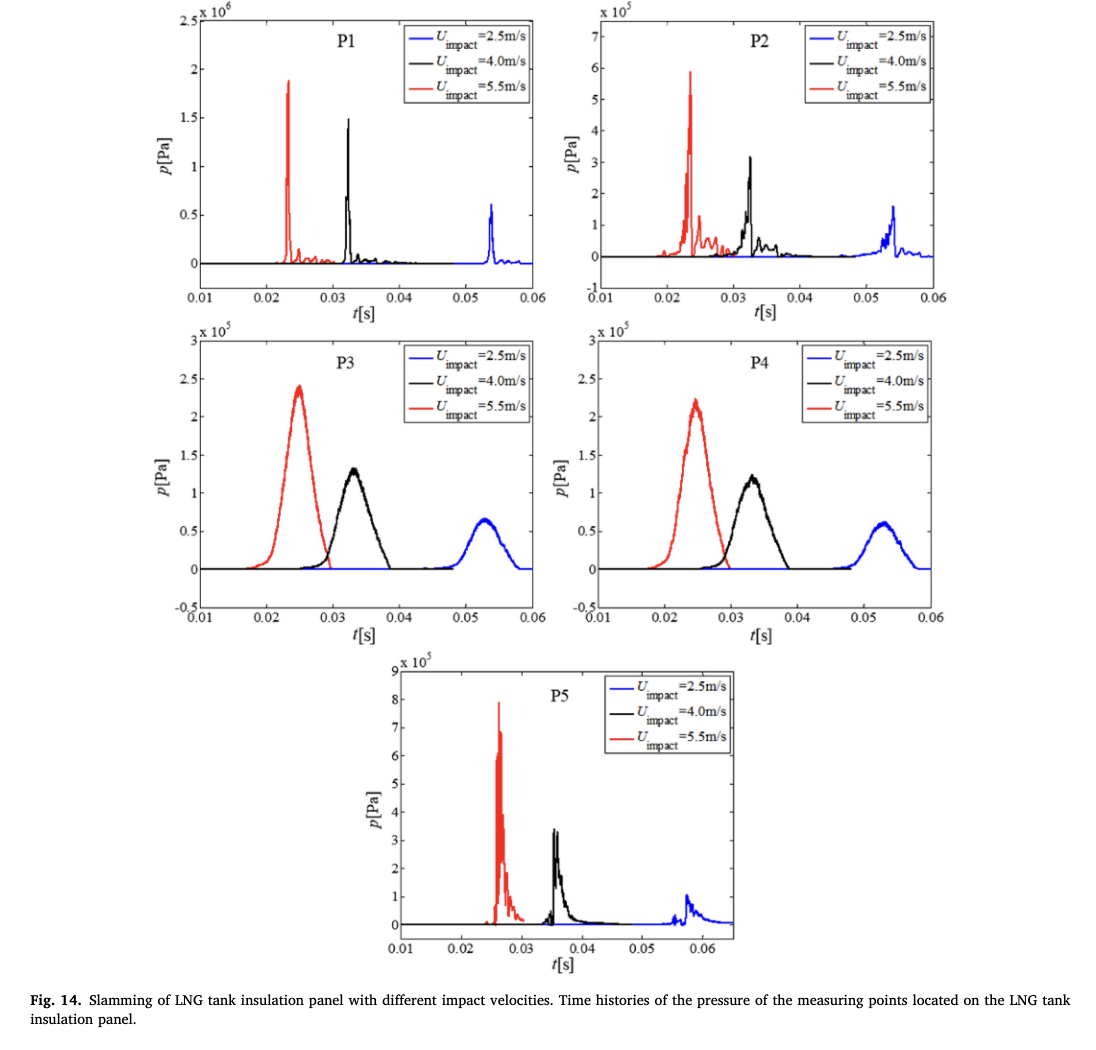
\includegraphics[width=30em]{./source/Fig14.png}
}

\subsubsection{Influence of the deadrise angle on slamming of LNG tank insulation panel-静升角对LNG船绝缘板砰击的影响}
\paragraph{\quad}In this subsection, the water slamming of the LNG tank insulation panel with different 
                deadrise angles is simulated, and the influence of the deadrise angle on the slamming load is analyzed. 
                The mass and initial impact velocity of the plate remain the same as those in subsection 3.2.1. Taking 
                the left dent of the panel as center, the initial deadrise angle of the LNG tank insulation panel is 
                adjusted to θ = 2◦ and θ = 6◦, respectively. Fig. 15 displays the particle distributions of the water 
                slamming of LNG tank insulation panel with different deadrise angles. It can be observed that for the 
                insulation panel with smaller deadrise angle, more air under the panel will be trapped, and therefore a 
                larger air bubble is generated under the panel. When the deadrise angle ranges from 2◦ to 6◦, the air bubble 
                under the panel with larger deadrise angle is closer to the right side. In addition, different from the panels 
                with deadrise angles of 2◦ and 4◦, for the panel with deadrise angle of 6◦, a small air cushion is formed 
                between the left corner and the left dent of the panel when its left corner impacts the water as shown in 
                the red box in Fig. 15, and then overflows the water from the left corner.
\paragraph{\quad}在这一小节中,模拟了不同静升角下的LNG船绝缘板与水的砰击,并分析了静升角对砰击载荷的影响。
                板的质量和初始砰击速度保持与subsection 3.2.1中相同。以板的左齿为中心,调整LNG船绝缘板的初始静升角分别为$\theta = 2^\circ$
                和$\theta = 6^\circ$。Fig. 15给出了不同静升角的LNG船绝缘板与水砰击的粒子分布。可以看出越小的静升角的绝缘板能够困住更多
                的空气,因此板底生成了更大的气泡。当静升角从$2^\circ$到#$6^\circ$,越大的静升角下的板底的气泡越靠近右侧。
                此外,与静升角$2^\circ$和$4^\circ$下的板不同,对于静升角$6^\circ$,当左角砰击水面时,在左角和左齿间形成了一个更小的气垫,如
                Fig. 15红框所示,随后从左角溢出水。\\
{
    \centering
    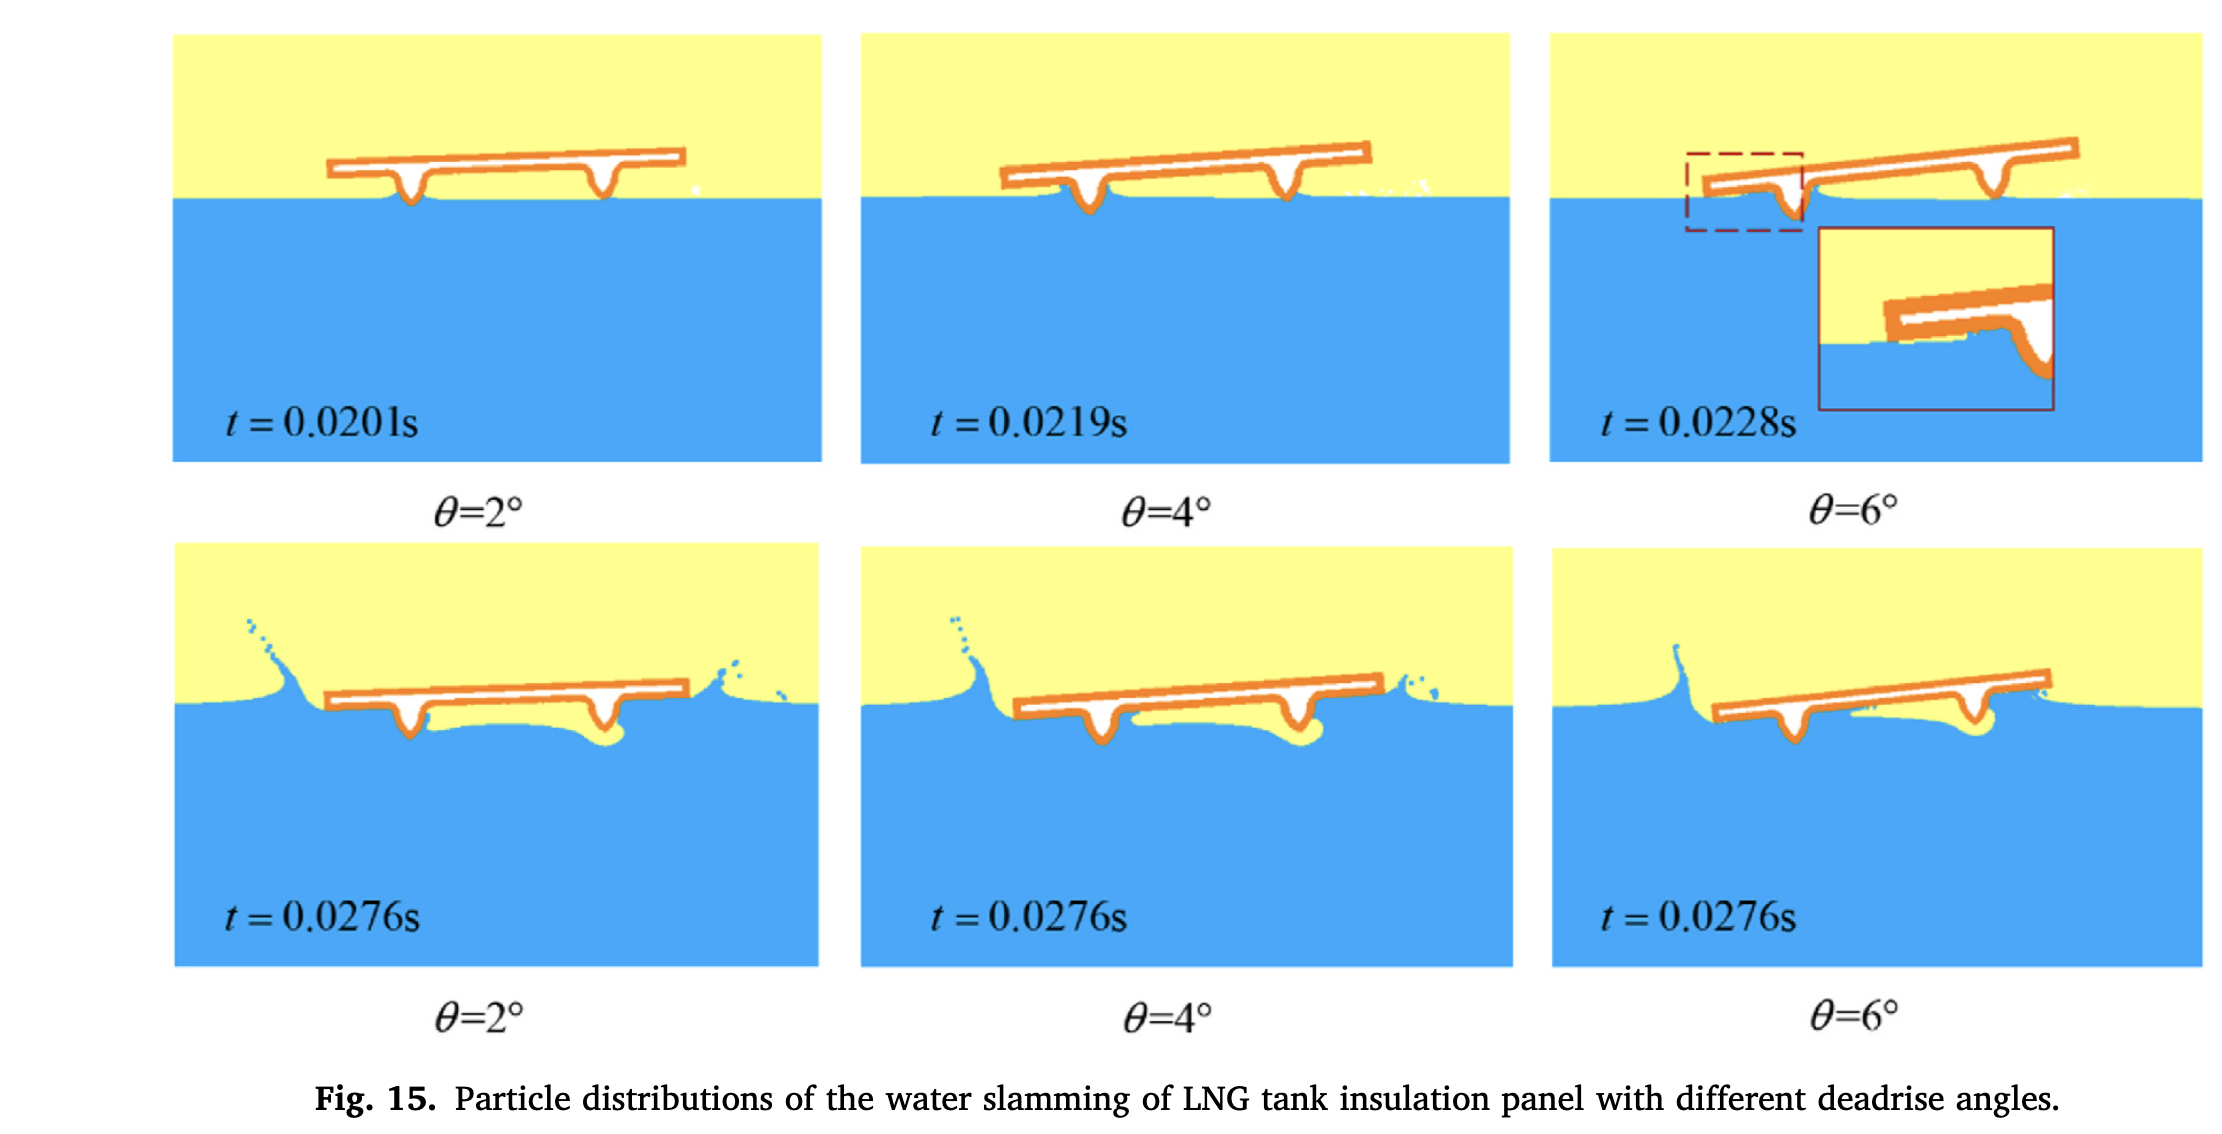
\includegraphics[width=30em]{./source/Fig15.png}
}

\paragraph{\quad}Fig. 16 gives the time histories of the pressure of the five measuring points on the panel 
                with different deadrise angles. It can be found that generally, the slamming pressure peak 
                of the point on the panel with a smaller deadrise angle is lower. Specifically, for points 
                P3, P4 and P5, because the larger deadrise angle makes these measuring points on panel farther 
                from the water surface, it is found that the time histories of pressure of these measuring 
                points on the panel with a larger deadrise angle are more lagging with a larger peak. 
                In particular, for points P3 and P4, the pulse width of their time histories of pressure on 
                the panel with larger deadrise angle is significantly reduced due to the smaller air bubble 
                formed under the plate. For points P1 and P2, the pressure peak of the panel with a larger 
                deadrise angle appears earlier. However, for point P1, the variation trend of its pressure 
                peak is different. It can be found that the pressure peak of the panel with the deadrise angle 
                of 6◦ is smaller than that of the panel with the deadrise angle of 4◦ and close to that of the 
                panel with the deadrise angle of 2◦ owing to the small air cushion formed below the point P1.
\paragraph{\quad}Fig. 16给出了不同静升角下板上五个测量点压力的时间历程。可以发现通常情况下,静升角越小的板的砰击压力峰值越小。
                具体来说,对于点P3,P4,P5,因为越大的静升角使这些测量低与水面越远,可以发现越大静升角上测量点的时间历程有越大且越滞后的压力峰值。
                特别地,对于点P3和P4,由于板下形成的气泡越小,越大的静升角其板上压力的时间历程的脉冲宽度大幅减小。对于点P1和P2,更大
                静升角的板的压力峰值出现得更早。然而,对点P1,其压力峰值的变化趋势是不同的。可以看出静升角$6^\circ$下板压力峰值小于
                静升角$4^\circ$下板的压力峰值,并接近静升角$2^\circ$下板的压力峰值,这是因为点P1下形成的小气垫。\\
{
    \centering
    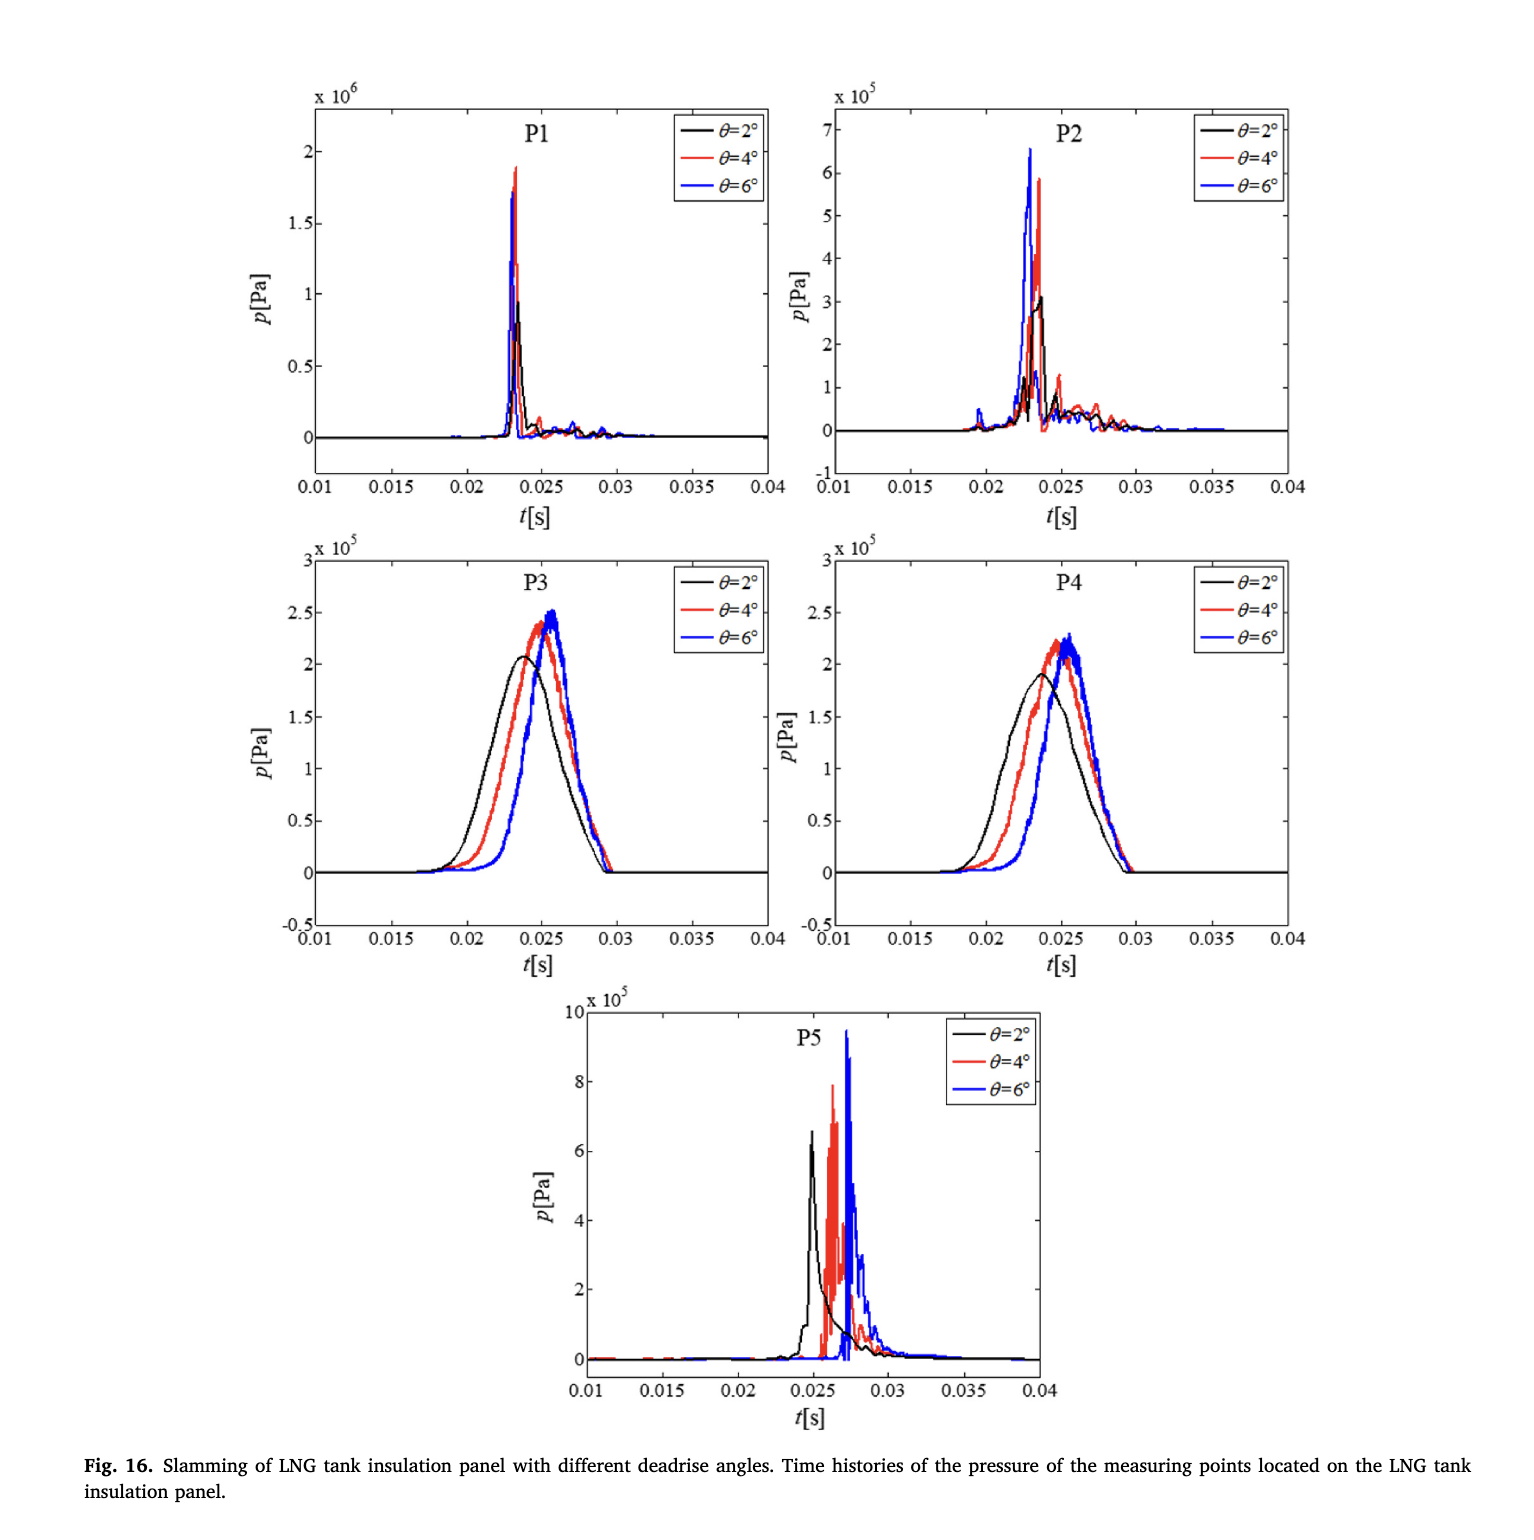
\includegraphics[width=30em]{./source/Fig16.png}
}

\end{document}